\chapter{Arhitektura i dizajn sustava}
	\textit{Arhitektura cijelog sustava može se podijeliti na četiri ključna dijela:}
		\begin{itemize}
    		\item Web preglednik
    		\item Web aplikacija
    		\item Baza podataka
    		\item Code runner
		\end{itemize}

	\textit{\underline{Web preglednik} omogućuje interakciju između korisnika i aplikacije. Svaki se korisnikov zahtjev
	 događa na web pregledniku i prosljeđuje aplikaciji na obradu. Osim slanja zahtjeva, korisniku se omogućuje
	  bolji pregled aplikacije pomoću apstraktnog koda kojeg web preglednik pretvara u lako shvatljive strukture.}\\

	\textit{\underline{Aplikacija} se sastoji od dva glavna dijela, frontenda i backenda. Tehnologije koje se koriste na backendu
	 uključuju programski jezik \textbf{Python} i \textbf{fastApi} web framework koji omogućuje stvaranje aplikacije temeljene na \textbf{REST}
	 arhitekturi i rutera na kojem su definirane rute za slanje zahtjeva i komunikaciju korisnika i aplikacije.
	 Frontend aplikacije izrađen je korištenjem JavaScript librarya \textbf{React}. On omogućuje korisniku jednostavan pregled
	 aplikacije i jednostavno korištenje aplikacije, odnosno slanje zahtjeva.}\\

	\textit{\underline{Kontejneri} se koriste unutar aplikacije kako bi poboljšali korisničko iskustvo, optimizirali performanse sustava
	te osigurali skalabilnost za povećani broj korisnika. Glavni se dio aplikacije s ruterima i logikom za komunikaciju s 
	bazom nalazi u vlastitom kontejneru kao i glavna baza, evaluator i blob storage.}\\

	\textit{Za \underline{bazu podataka} se koristi \textbf{SQL} specifično \textbf{PostgreSQL}. Glavna baza se nalazi u vlastitom kontejneru kojemu backend
	aplikacije pristupa kako bi spremio informacije u nju. Na backendu se koristi \textbf{psycopg} PostgreSQL adapter koji omogućuje
	komunikaciju između baze i backenda.}\\
	
	\textit{\underline{Evaluator} komunicira s vanjskim \underline{Code runnerom} za kompajliranje kodova koje korisnik šalje
	na backend. Ovaj ključni dio sustava odgovoran je za izvršavanje kôda unutar sigurnog okruženja, čime se osigurava
	izolacija korisničkih skripti od ostatka aplikacije. Kroz ovu komunikaciju, Evaluator prima kôd od korisnika,
	proslijeđuje ga Code runneru na izvršavanje te zatim interpretira rezultate kako bi ih pravilno integrirao
	natrag u aplikaciju.}

	\textit{Dodatno, evaluator koristi \textbf{blob storage} pomoću kojeg dohvaća podatke koji su mu potrebni za
	evaluaciju određenog zadatka. Evaluator ima pristup informacijama poput ulaznih podataka za testiranje,
	očekivanih rezultata te drugih specifičnih parametara vezanih uz pojedini zadatak.}
	
	\newpage
	
		

		

				
		\section{Baza podataka}
			
		Za implementaciju našeg sustava koristit ćemo PostgreSQL, relacijsku bazu podataka. Ovaj tip baze podataka posebno je pogodan za modeliranje kompleksnih struktura koje odražavaju realni svijet, zahvaljujući svojoj sposobnosti da efikasno upravlja relacijama, odnosno tablicama. Svaka tablica u bazi unikatno je definirana svojim nazivom i skupom atributa, čime se omogućava precizno strukturiranje podataka. Jedna od ključnih prednosti PostgreSQL baze je njena brzina i efikasnost u obradi podataka, uključujući pohranu, ažuriranje i dohvaćanje informacija. Naša baza podataka obuhvatit će niz entiteta koji su specifično prilagođeni zahtjevima naše aplikacije.
		Popis entiteta: users, competitions, problems, competition_participations, problems_on_competitions, problem_results, trophies i verification_tokens.
			\subsection{Opis tablica}
			

				\textit{Svaku tablicu je potrebno opisati po zadanom predlošku. 
				Lijevo se nalazi točno ime varijable u bazi podataka, u sredini se nalazi tip podataka, 
				a desno se nalazi opis varijable. Svjetlozelenom bojom označite primarni ključ. Svjetlo plavom označite strani ključ}
				
				
				\subsubsection*{Users}
				
				Entitet \bold{users} sadržava sve važne informacije o korisniku aplikacije. Sadrži atribute: \textit{id, role, username, image_url, password_hash, email, name, surname, is\_verified, created\_on}. Ovaj entitet je u \textit{many to many} vezi s entitetom \textit{competitions} preko tablice \textit{competition\_participations}. Ovaj entitet je u \textit{one to many} vezi s entitetom \textit{verification\_tokens} preko atributa \textit{email}. 
				\vspace{20mm}

				\begin{figure}[htbp]
					\centering
					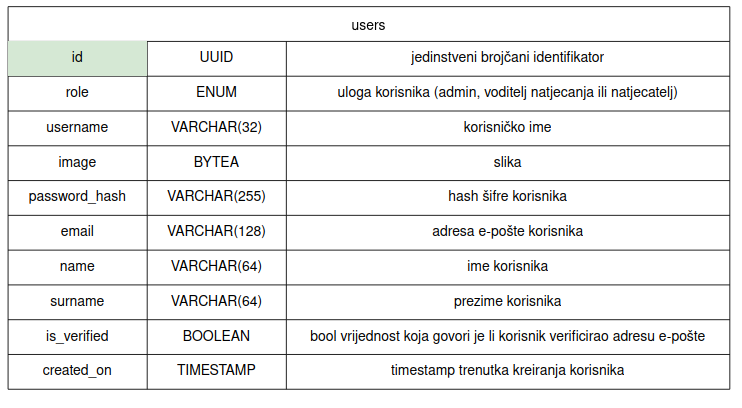
\includegraphics[width=\linewidth]{slike/users_tablica.png}
				\end{figure}

				\vspace{30mm}

				\subsubsection*{Problems}

				Entitet \bold{problems} sadržava sve važne informacije o zadacima. Sadržava atribute: \textit{id, name, description, example\_input, example\_output, is\_hidden, num\_of\_points, runtime\_limit, description, tests\_dir, is_\_private, created\_on}. Ovaj entitet je u \textit{many to many} vezi s entitetom \textit{competitions} preko tablice \textit{problems\_on\_competitions}. Ovaj entitet je u \textit{one to many} vezi s entitetom \textit{problem\_results} preko atributa \textit{id}.

				\vspace{20mm}

				\begin{figure}[htbp]
					\centering
					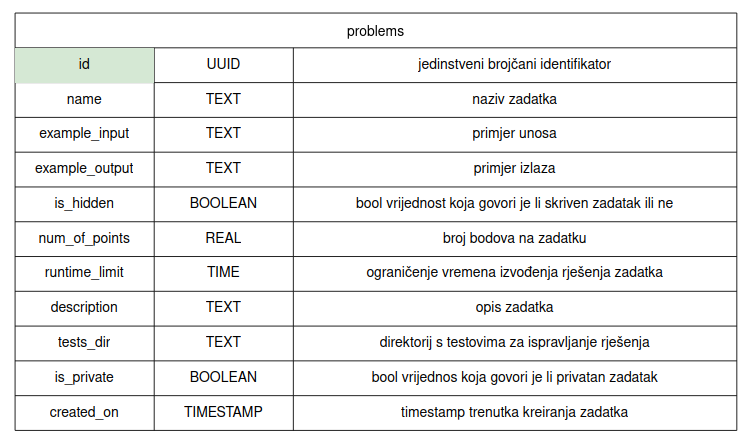
\includegraphics[width=\linewidth]{slike/problems_tablica.png}
				\end{figure}

				\vspace{30mm}

				\subsubsection*{Competitions}

				Entitet \bold{competitions} sadržava sve važne informacije o natjecanjima. Sadržava atribute: \textit{id, name, description, start\_time, end\_time, parent\_id, problems}. Natjecanja mogu imati svoja nadređena natjecanja. Ovaj entitet je u \textit{many to many} vezi s users entitetom preko competition\_participations tablice. Ovaj entitet je u \textit{many to many} vezi s problems entitetom preko problems\_on\_competitions tablice.                          
			
				\vspace{20mm}

				\begin{figure}[htbp]
					\centering
					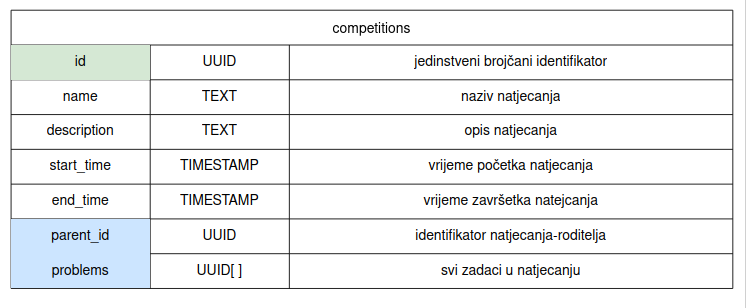
\includegraphics[width=\linewidth]{slike/competitions_tablica.png}
				\end{figure}

				\vspace{30mm}

				\subsubsection*{Competition\_participations}

				Entitet \bold{competition\_participations} sadržava sve važne informacije o sudjelovanju korisnika na natjecanjima. Sadržava atribute: \textit{id, user\_id, competition\_id, num\_of\_points}. Ovaj entitet je u \textit{many to many} vezi s users entitetom. Ovaj entitet je u \textit{many to many} vezi s competitions entitetom preko atributa \textit{competition\_id}.

				\vspace{20mm}

				\begin{figure}[htbp]
					\centering
					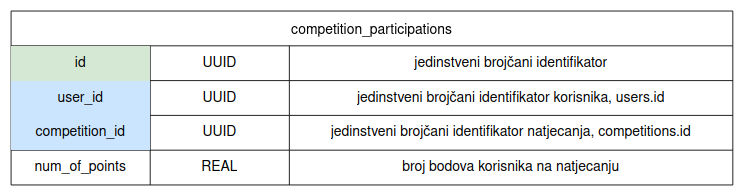
\includegraphics[width=\linewidth]{slike/competition_participations_tablica.png}
				\end{figure}

				\vspace{30mm}

				\subsubsection*{Problems\_on\_competitions}

				Entitet \bold{problems\_on\_competitions} sadržava informacije o zadacima koji pripadaju pojedinim natjecanjima. Sadržava atribute: \textit{id, problem\_id, competition\_id, num\_of\_points}.

				\vspace{20mm}

				\begin{figure}[htbp]
					\centering
					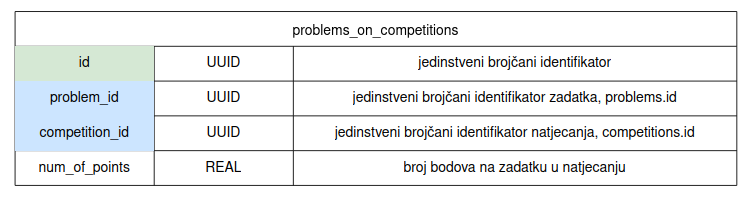
\includegraphics[width=\linewidth]{slike/problems_on_competitions_tablica.png}
				\end{figure}

				\vspace{30mm}

				\subsubsection*{Problem\_results}

				\vspace{20mm}

				Entitet \bold{problems\_results} sadrži rezultate pojedinih korisnika na pojedinim zadacima. Sadržava atribute: \textit{id, user\_id, problem\_id, competition\_id, num\_of\_points, average\_runtime, is\_correct, source\_code} i\textit{one to many} vezi s users entitetom preko users\_id te \textit{one to many} vezi s problems entitetom preko atributa \textit{problem\_id}. Ovaj entitet je u \textit{one to many} vezi s competitions entitetom preko atributa \textit{competition\_id}.

				\vspace{20mm}

				\begin{figure}[htbp]
					\centering
					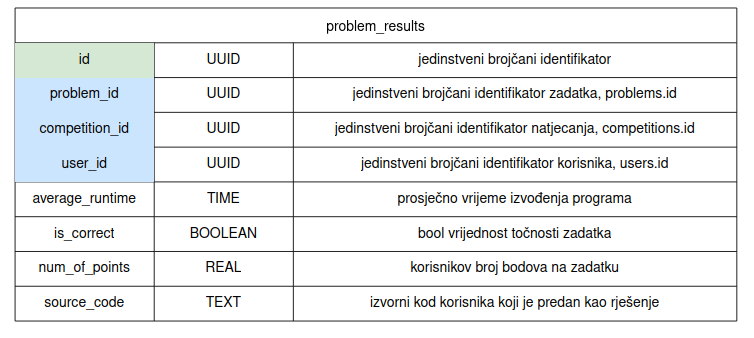
\includegraphics[width=\linewidth]{slike/problem_results_tablica.png}
				\end{figure}

				\vspace{30mm}

				\subsubsection*{Trophies}

				Entitet \bold{trophies} sadržava informacije o trofejima koje korisnici mogu osvojiti. Sadržava atribute: \textit{id, competition\_id, user\_id, position, icon }. Ovaj entitet je u \textit{one to many} vezi s users entitetom preko atributa \textit{user\_id} te \textit{one to many} vezi s competitions entitetom preko atributa \textit{competition\_id}.
			
				\vspace{20mm}

				\begin{figure}[htbp]
					\centering
					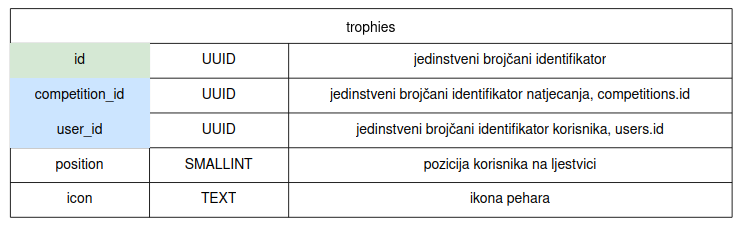
\includegraphics[width=\linewidth]{slike/trophies_tablica.png}
				\end{figure}

				\vspace{30mm}

				\subsubsection*{Verification\_tokens}

				Entitet \bold{verification\_tokens} sadržava informacije o tokenima za verifikaciju korisnika. Sadržava atribute: \textit{token, email, expiry\_date}. Ovaj entitet je u \textit{one to many} vezi s users entitetom preko atributa \textit{email}.

				\vspace{20mm}

				\begin{figure}[htbp]
					\centering
					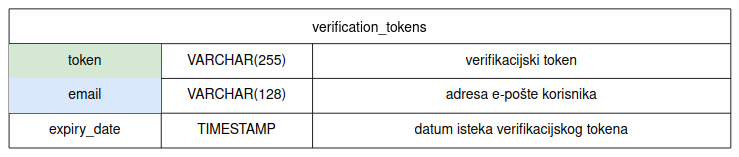
\includegraphics[width=\linewidth]{slike/verification_tokens_tablica.png}
				\end{figure}

				\vspace{30mm}

				\clearpage
				\subsection{Dijagram baze podataka}
				\textit{ U ovom potpoglavlju potrebno je umetnuti dijagram baze podataka. Primarni i strani ključevi moraju biti označeni, a tablice povezane. Bazu podataka je potrebno normalizirati. Podsjetite se kolegija "Baze podataka".}
				vspace{20mm}

				\begin{figure}[htbp]
					\centering
					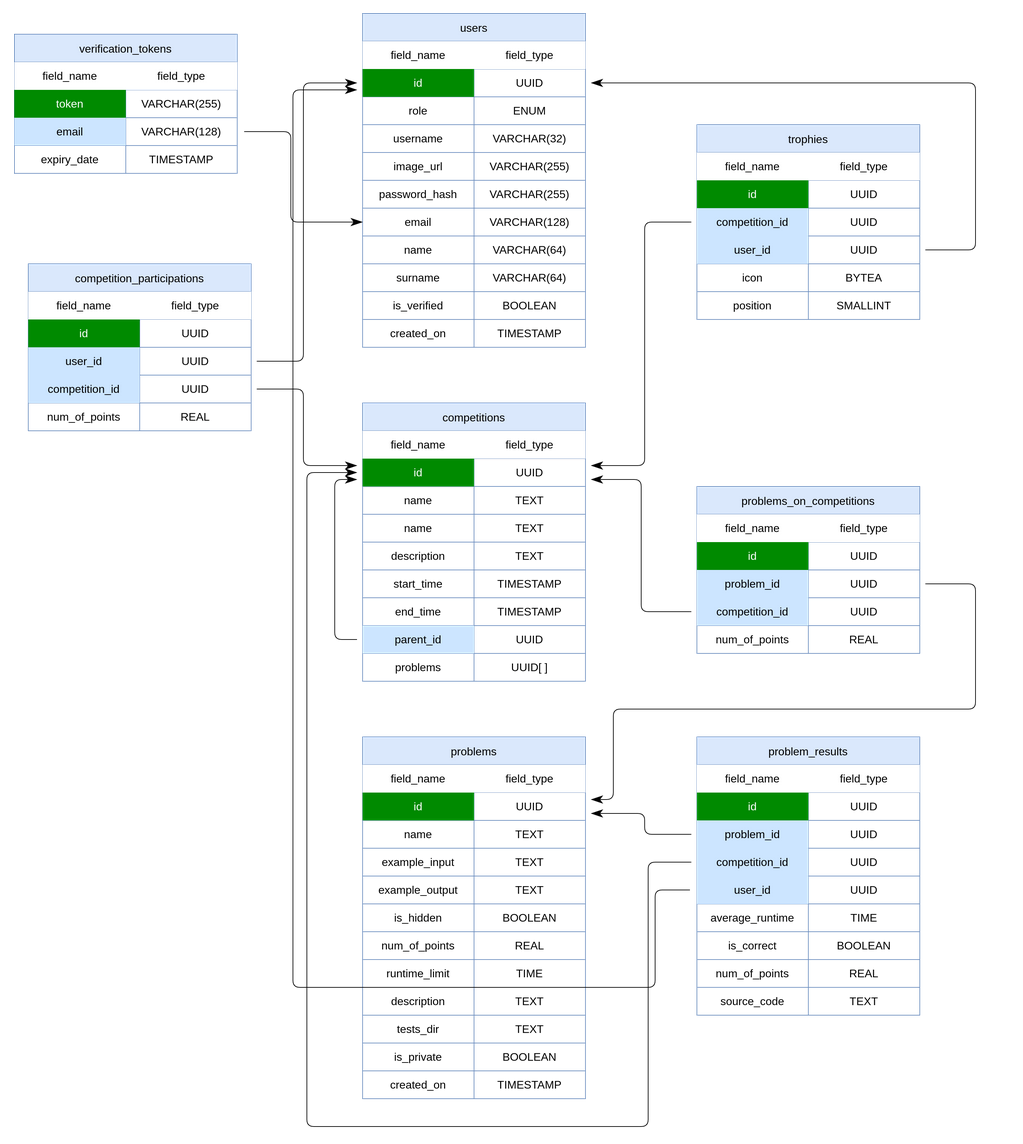
\includegraphics[width=\linewidth]{slike/db_dijagram.png}
				\end{figure}

			\eject
			
			
		\section{Dijagram razreda}
		
			\textit{Potrebno je priložiti dijagram razreda s pripadajućim opisom. Zbog preglednosti je moguće dijagram razlomiti na više njih, ali moraju biti grupirani prema sličnim razinama apstrakcije i srodnim funkcionalnostima.}\\
			
			Na sljedećim slikama prikazani su dijagrami razreda koji pripadaju backend dijelu aplikacije.
			
			\begin{figure}[htbp]
				\centering
				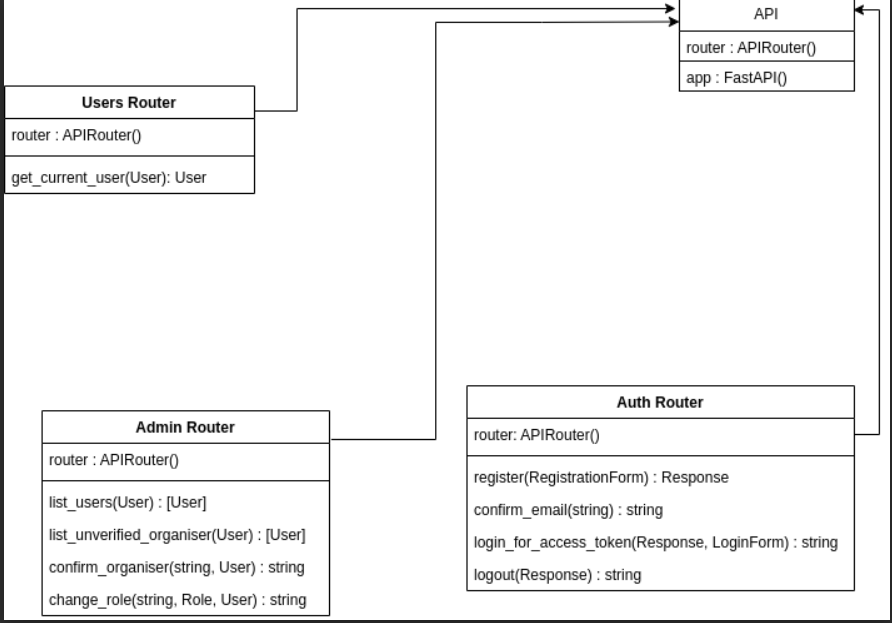
\includegraphics[width=\linewidth]{slike/dijagram_razreda.png}
			\end{figure}

			\begin{figure}[htbp]
				\centering
				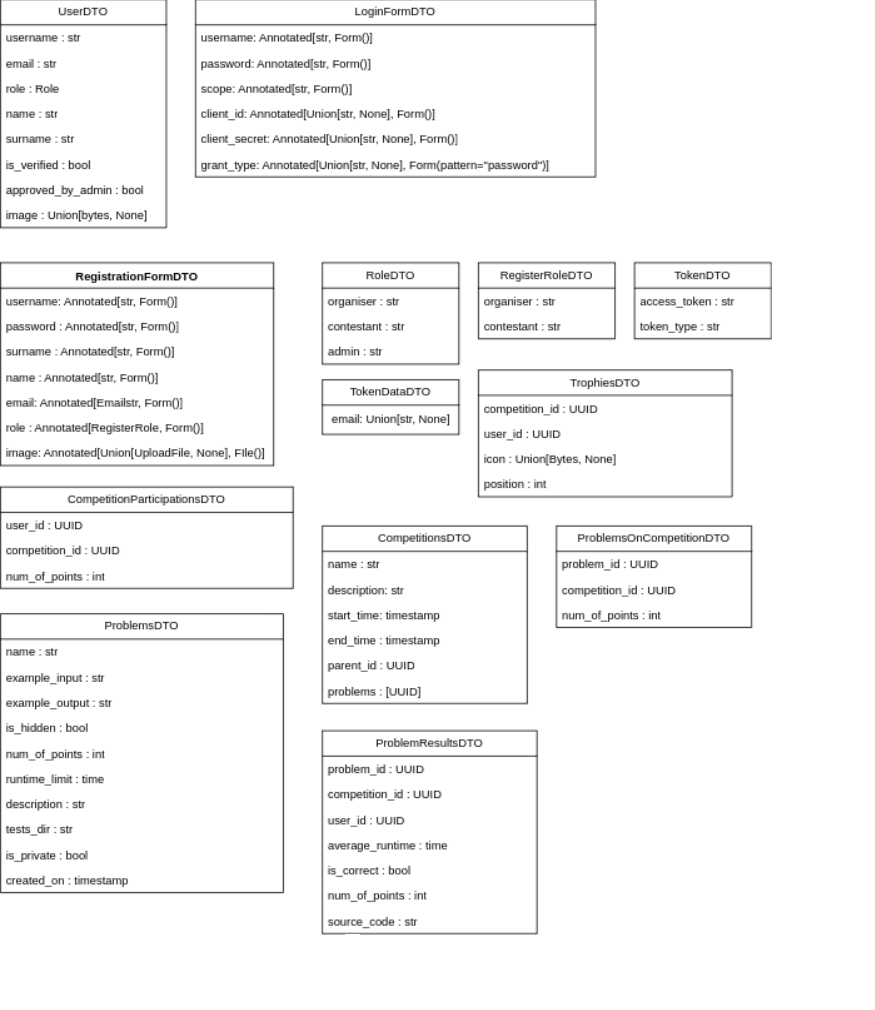
\includegraphics[width=\linewidth]{slike/dto.png}
			\end{figure}

			\textbf{\textit{dio 1. revizije}}\\
			
			\textit{Prilikom prve predaje projekta, potrebno je priložiti potpuno razrađen dijagram razreda vezan uz \textbf{generičku funkcionalnost} sustava. Ostale funkcionalnosti trebaju biti idejno razrađene u dijagramu sa sljedećim komponentama: nazivi razreda, nazivi metoda i vrste pristupa metodama (npr. javni, zaštićeni), nazivi atributa razreda, veze i odnosi između razreda.}\\
			
			\textbf{\textit{dio 2. revizije}}\\			
			
			\textit{Prilikom druge predaje projekta dijagram razreda i opisi moraju odgovarati stvarnom stanju implementacije}
			
			
			
			\eject
		
		\section{Dijagram stanja}
			
			
			\textbf{\textit{dio 2. revizije}}\\
			
			\textit{Potrebno je priložiti dijagram stanja i opisati ga. Dovoljan je jedan dijagram stanja koji prikazuje \textbf{značajan dio funkcionalnosti} sustava. Na primjer, stanja korisničkog sučelja i tijek korištenja neke ključne funkcionalnosti jesu značajan dio sustava, a registracija i prijava nisu. }
			
			
			\eject 
		
		\section{Dijagram aktivnosti}
			
			\textbf{\textit{dio 2. revizije}}\\
			
			 \textit{Potrebno je priložiti dijagram aktivnosti s pripadajućim opisom. Dijagram aktivnosti treba prikazivati značajan dio sustava.}
			
			\eject
		\section{Dijagram komponenti}
		
			\textbf{\textit{dio 2. revizije}}\\
		
			 \textit{Potrebno je priložiti dijagram komponenti s pripadajućim opisom. Dijagram komponenti treba prikazivati strukturu cijele aplikacije.}